\chapter{Objekte im Raum}
\begin{inhalt}
  \begin{itemize}
    \item Geraden
    \item Ebenen: Parameter-, Normalen-, Koordinatendarstellung
    \item Darstellungsformen untereinander umformen
  \end{itemize}
\end{inhalt}

\begin{bla}{Geraden}
  %
  \begin{marginfigure}[0em]
    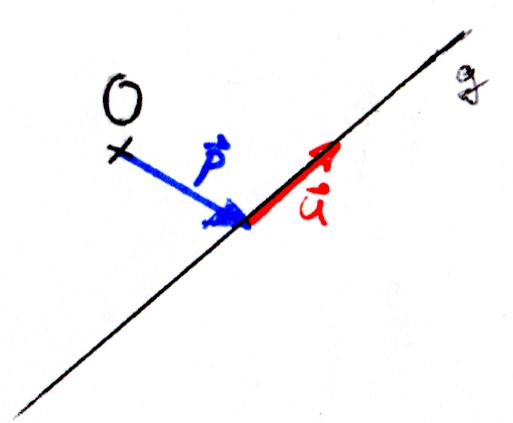
\includegraphics[scale=0.8]{AGLage_Gerade}
    \caption{Gerade, Richtung $\vec{u}$, stützt sich auf $\vec{p}$}
  \end{marginfigure}
  %
  Eine Gerade g die durch den Punkt $P$ in Richtung $\vec{u}$ läuft kann geschrieben werden als:
  \begin{equation*}
    \text{g: }\ \vec{x} = \vec{p} + \text{r} * \vec{u}\text{, mit r}\in\R
  \end{equation*}
  Die Vorstellung dazu ist, dass man alle Punkte $\vec{x}$ auf der Geraden trifft, indem man von $P$ aus den Vektor $\vec{u}$ verlängert oder verkürzt.
\end{bla}

\begin{bla}{Ebenen - Parameterdarstellung}
  %
  \begin{marginfigure}[0em]
    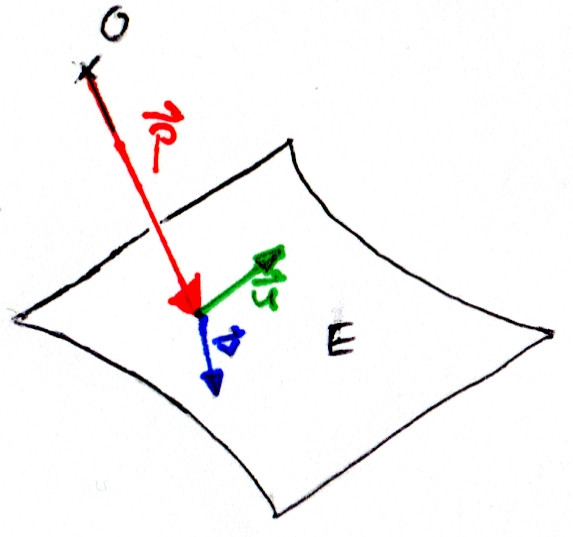
\includegraphics[scale=0.8]{AGLage_EbeneParam}
    \caption{Ebene, aufgespannt durch $\vec{u}$ und $\vec{v}$, stützt sich auf $\vec{p}$}
  \end{marginfigure}
  %
  Genauso kann man auch Ebenen darstellen, nur dass man von $P$ aus in zwei Richtungen gehen kann:
  \begin{equation*}
    \text{E: }\ \vec{x} = \vec{p} + \text{r} * \vec{u} + \text{s} * \vec{v} \text{, mit r, s} \in \R
  \end{equation*}
  $\vec{u}$ und $\vec{v}$ nennt man \emph{Spannvektoren} der Ebene E.
\end{bla}

\begin{bla}{Ebenen - Normalendarstellung}
  %
  \begin{marginfigure}[0em]
    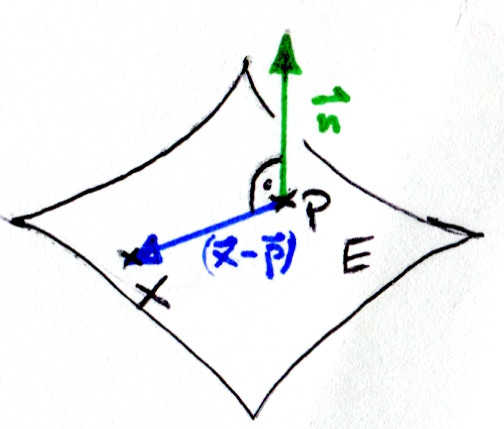
\includegraphics[scale=0.8]{AGLage_EbeneNormal}
    \caption{Ebene senkrecht zu $\vec{n}$, ausgehend von Stützpunkt $P$}
  \end{marginfigure}
  %
  Zu jeder Ebene gehört ein Vektor, der senkrecht darauf steht.

  Der sogenannte \emph{Normalenvektor} steht dann auch senkrecht auf allen Linien, die in der Ebene liegen.

  Eine Ebene E beschreibt man damit wie folgt:
  \begin{equation*}
    \text{E: }\ \left( \vec{x} - \vec{p} \right) * \vec{n} = 0
  \end{equation*}
  $\vec{x} - \vec{p}$ ist die Verbindung $\overrightarrow{PX}$ zwischen X und der Stützstelle P.
  Diese Verbindung liegt in der Ebene, und steht damit senkrecht auf $\vec{n}$. Das Skalarprodukt ist Null.
\end{bla}



\begin{bla}{Ebenen - Koordinatendarstellung}
  \label{AG:E-Koordinatendarst}
  Wenn man die Normalendarstellung ausmultipliziert, ergibt sich folgende Gleichung für E:
  \begin{align*}
    \vec{x} * \vec{n} &= \vec{p} * \vec{n}\\
    n_1*x_1 + n_2*x_2 + n_3*x_3 &= c
  \end{align*}
  $\vec{p} * \vec{n}$ lässt sich ausrechnen und ergibt die Zahl $c$.

  Diese Darstellung ist nicht so offensichtlich aus Vektoren aufgebaut, aber sehr hilfreich um einige Aufgaben auszurechnen.
\end{bla}

\begin{bla}{Ebenen - \textsc{Hesse}'sche Normalenform}
  Die Gleichungen der Normalen- und Koordinatendarstellung können durch den Betrag des Normalenvektors geteilt werden:
  \begin{align*}
    \text{E: }\ \frac{ \left(n_1*x_1 + n_2*x_2 + n_3*x_3\right)}{|\vec{n}|} - \frac{c}{|\vec{n}|}
    &=
    0
    \\
    \text{E: }\ \frac{\left( \vec{x} - \vec{p} \right) * \vec{n}}{|\vec{n}|}
    &=
    0
  \end{align*}

  Die Darstellung wird im nächsten Kapitel sehr praktisch zur Abstandsbestimmung sein.
\end{bla}

\section{Ebenengleichungen aus Punkten}
Gesucht werden im Folgenden die Ebenengleichungen wenn drei Punkte $A,B,C$ beziehungsweise $\vec{a}, \vec{b}, \vec{c}$ im Raum gegeben sind.

\begin{bla}{Stützvektor}
  Der Stützvektor muss einfach irgendeinen Punkt auf der Ebene treffen, also kann man zum Beispiel $\vec{a}$ aussuchen.
\end{bla}

\begin{bla}{Spannvektoren}
  Die Spannvektoren sind irgendwelche zwei Vektoren, die in der Ebene oder parallel dazu laufen. Wir haben zur Auswahl: $\overrightarrow{AB}$, $\overrightarrow{BC}$ und $\overrightarrow{AC}$.

  \textbf{Wichtig: Lineare Unabhängigkeit:} Wenn nur zwei Punkte gegeben sind, oder die drei Punkte auf einer Geraden liegen haben wir nicht genügend verschiedene Vektoren um eine Ebene zu basteln.
  Man erkennt das daran, dass die Vektoren in die gleiche Richtung zeigen, nur verschieden lang sind
  (Das Kreuzprodukt ist dann Null).
\end{bla}

\begin{bla}{Normalenvektor}
  Kennt man schon zwei verschiedene Spannvektoren, bekommt man den Normalenvektor über deren Kreuzprodukt.

  Man kann stattdessen aber auch die Koordinatengleichung für Ebenen benutzen:
  \begin{equation*}
    n_1x_1 + n_2x_2 + n_3x_3 = b
  \end{equation*}



  Setzt man jetzt zum Beispiel die Punkte $A=(1|1|0), B=(1|0|1), C=(0|0|1)$ für $\vec{x}$ ein, ergeben sich die Gleichungen:
  \begin{align*}
    n_1 + n_2 &= b \\
    n_1 + n_3 &= b \\
    n_2 + n_3 &= b \\
    \text{Es folgt: } n_1 = n_2 = n_3 &= \frac{1}{2} * b
  \end{align*}
  Man wählt dann $b$ irgendwie und hat nicht nur den Normalenvektor, sondern gleich die dazu passende Koordinatengleichung.
\end{bla}

So konstruiert man die Koordinatengleichung, für die beiden anderen Gleichungen muss man nur die entsprechenden Vektoren an der richtigen Stelle einsetzen.

\section{Ebenengleichungen aus Ebenengleichungen}
\begin{bla}{Parameter- zu Normalenform}
  Eine Parameterform ist gegeben:
  \[
  \text{E: }\ \vec{p} + r * \vec{u} + s * \vec{v} \text{, mit }r,s \in \R
  \]
  Für die Normalenform brauchen wir einen Normalenvektor $\vec{n}$, der senkrecht auf den beiden Spannvektoren steht: $\vec{n} * \vec{u} = 0$ und $\vec{n}*\vec{v} = 0$

  Die Spannvektoren sind bekannt, also kann man die Gleichungen ausmultiplizieren und bekommt ein LGS für $n_1, n_2$ und $ n_3$.
  Zwei Gleichungen für drei Variablen liefern kein eindeutiges Ergebnis, also muss man am Schluss eine der drei Variablen selbst festlegen.

  Stattdessen kann man auch einfach $\vec{u} \times \vec{v} = \vec{n}$ ausrechnen.

  Der Stützvektor kann gleich bleiben.
\end{bla}

\begin{bla}{Koordinaten- zu Normalenform}
  \label{5_UmformungKN}
  Die Vorfaktoren vor den $x$-Werten sind die Komponenten des Normalenvektors.

  Um einen Stützvektor zu finden setzt man in der Koordinatenform ein paar $x$-Werte zu irgendeiner festen Zahl, so dass man einen Punkt ablesen kann.
  \begin{align*}
    x_1 + 2*x_2 -2 * x_3 &= 5\\
    \text{Setze $x_2 = 2$ und $x_3 = 0$: }\ x_1 + 4 &= 5\\
    \text{Es ergibt sich: } \vec{p} =
    \begin{pmatrix}
      x_1\\x_2\\x_3
    \end{pmatrix}
    &=
    \begin{pmatrix}
      1 \\ 2 \\ 0
    \end{pmatrix}
  \end{align*}
\end{bla}

\begin{bla}{Normalen- zu Koordinatenform}
  Das Skalarprodukt wird ausmultipliziert (siehe \ref{AG:E-Koordinatendarst}).
\end{bla}



\begin{bla}{Koordinaten- zu Parameterdarstellung}
  Einen Stützvektor findet man wie in \ref{5_UmformungKN} durch Einsetzen.

  Um Spannvektoren zu bekommen, suchen wir alle Vektoren $\vec{v}$, die auf $\vec{n}$ senkrecht stehen:
  \begin{align*}
    \vec{v} * \vec{n} &= 0\\
    n_1v_1 + n_2v_2 + n_3v_3 &= 0
  \end{align*}
  Um nicht parallele Spannvektoren zu bekommen setzen wir oben zum Beispiel einmal $v_2 = 0, v_3 = 1$ und einmal $v_2 = 1, v_3 = 0$, lösen damit die Gleichung und erhalten zwei Spannvektoren.
\end{bla}
